\chapter{Preparation}
\label{ch.preparation}

\section{Calculate the depth resolution of the OCT-system performing the folloing steps}

\subsection{Calculate the central wavenumber $k_0$ and the broadness of the spectral envelope function $\Delta k$}

\begin{equation}
k_0=\frac{2\pi}{\lambda_0} \rightarrow \frac{\Delta k}{\Delta\lambda}=-\frac{2\pi}{\lambda_0^2} 
\label{eq:delta_k_herleitung}
\end{equation}

\begin{equation}
\Delta k=-\frac{2\pi}{\lambda_0^2}\Delta\lambda
\label{eq:delta_k}
\end{equation}

With $\Delta\lambda = 130$~nm and $\lambda_0=1310~$nm equation \ref{eq:delta_k} becomes
\comwo{wie schreib ich, dass das negative vorzeichen bei delta k hier wegf�llt}
\begin{equation}
k_0=\frac{2\pi}{1310~\mathrm{nm}}=4.80~\mathrm{\upmu m}^{-1}
\label{eq:k_0_wert}
\end{equation}
and
\begin{equation}
\Delta k = \frac{2\pi}{1310 ^2~\mathrm{nm}^2}\cdot130~\mathrm{nm}=0,48~\mathrm{\upmu m}^{-1}
\label{eq:delta_k_wert}
\end{equation}

\subsection{Calculate Foriertransformations-F....$=S(z)$with respect to $P$}
The spectral power envelope $S(k)$ is a rectalngle of height $P$.
\begin{equation}
S(k)=P\cdot r_{\Delta k}(k-k_0)
\label{eq:S_k}
\end{equation}
with the rectangular function 

\begin{equation}
r_{\Delta k}(k-k_0)=\begin{cases}
1,&\mathrm{for}~|k-k_0|\leq\frac{\Delta k}{2} \\
0,&\mathrm{for}~|k-k_0|>\frac{\Delta k}{2} 
\end{cases}
\label{eq:rect}
\end{equation}

% A fourier transformation of $S(k)$ leads to $\breve{S}(z)$:
% \begin{equation}
% S(k)=P\cdot r_{\Delta k}(k-k_0)\qquad\laplace\qquad \mathrm{e}^{-jzk_0}\cdot P\Delta k\mathrm{sinc}(z\frac{\Delta k}{2})=\breve{S}(z)
% \label{eq:Transformation}
% \end{equation}
% with sinc$(x)=\frac{\mathrm{sin}(x)}{x}$
% 
% 
% \comwo{Nochmal ohne Korrespondenz, sondern selbst gerechnet:... �berleg dir ob was davon und wenn ja welches richtig ist}

% A Fourier transformation of $S(k)$ leads to $\breve{S}(z)$. To performe the Fourier transformation the function $Y(k)$ is introduced.
% \begin{equation}
% S(k)=P\cdot r_{\Delta k}(k-k_0)=Y(k-k_0)
% \label{eq:hilfsunktion}
% \end{equation} 
% 
% 
\begin{equation}
S(k)=Y(k-k_0)\qquad \laplace \qquad \breve{Y}(z)\cdot\mathrm{e}^{-jzk_0}=\breve{S}(z)
\label{eq:verschiebung}
\end{equation}

\begin{equation}
Y(k)=P\cdot r_{\Delta k}(k)
\label{eq:Y_k}
\end{equation}

To transform $Y(k)$ from the momentum space into the position-space the following integral needs to be solved:

\begin{equation} 
\begin{split} 
\breve{Y}(z)=\frac{1}{\sqrt{2\pi}}\int^{\infty}_{-\infty}P\cdot r_{\Delta k}(k)\mathrm{e}^{jkz}\mathrm{d}k \\
=			\frac{1}{\sqrt{2\pi}}\int^{\frac{\Delta k}{2}}_{-\frac{\Delta k}{2}}P\cdot \mathrm{e}^{jkz}\mathrm{d}k\\
=			\frac{P}{\sqrt{2\pi}}\left[\frac{\mathrm{e}^{jkz}}{jz}\right]^{\frac{\Delta k}{2}}_{-\frac{\Delta k}{2}}\\
=		\frac{P}{\sqrt{2\pi}}\left(\frac{\mathrm{e}^{j\Delta kz}}{jz}-\frac{\mathrm{e}^{-j\Delta kz}}{jz}\right)\\
=		\frac{P}{\sqrt{2\pi}}\cdot\frac{2\mathrm{sin}(\frac{\Delta k}{2}z)}{z}\\
=		\frac{P}{\sqrt{2\pi}}\Delta k \cdot\mathrm{sinc}(\frac{\Delta k}{2}z)
\end{split}
\end{equation}

with sinc$(x)=\frac{\mathrm{sin}(x)}{x}$

With equation \eqref{eq:verschiebung} this leads to

\begin{equation}
\breve{S}(z) = \frac{P}{\sqrt{2\pi}}\Delta k \cdot\mathrm{sinc}(\frac{\Delta k}{2}z)\cdot\mathrm{e}^{-jzk_0}
\label{eq:S_ortsraum}
\end{equation}

\subsection{What is the FWHM of $\breve{S}(z)$?}

The determination of the FWHM of $\breve{S}(z)$ was done graphical. Figure \ref{fig:fwhm} shows the main peak of $\breve{S}(z)$. The measured FWHM is $\sim$16~nm. 
\begin{figure}[h]%
\centering
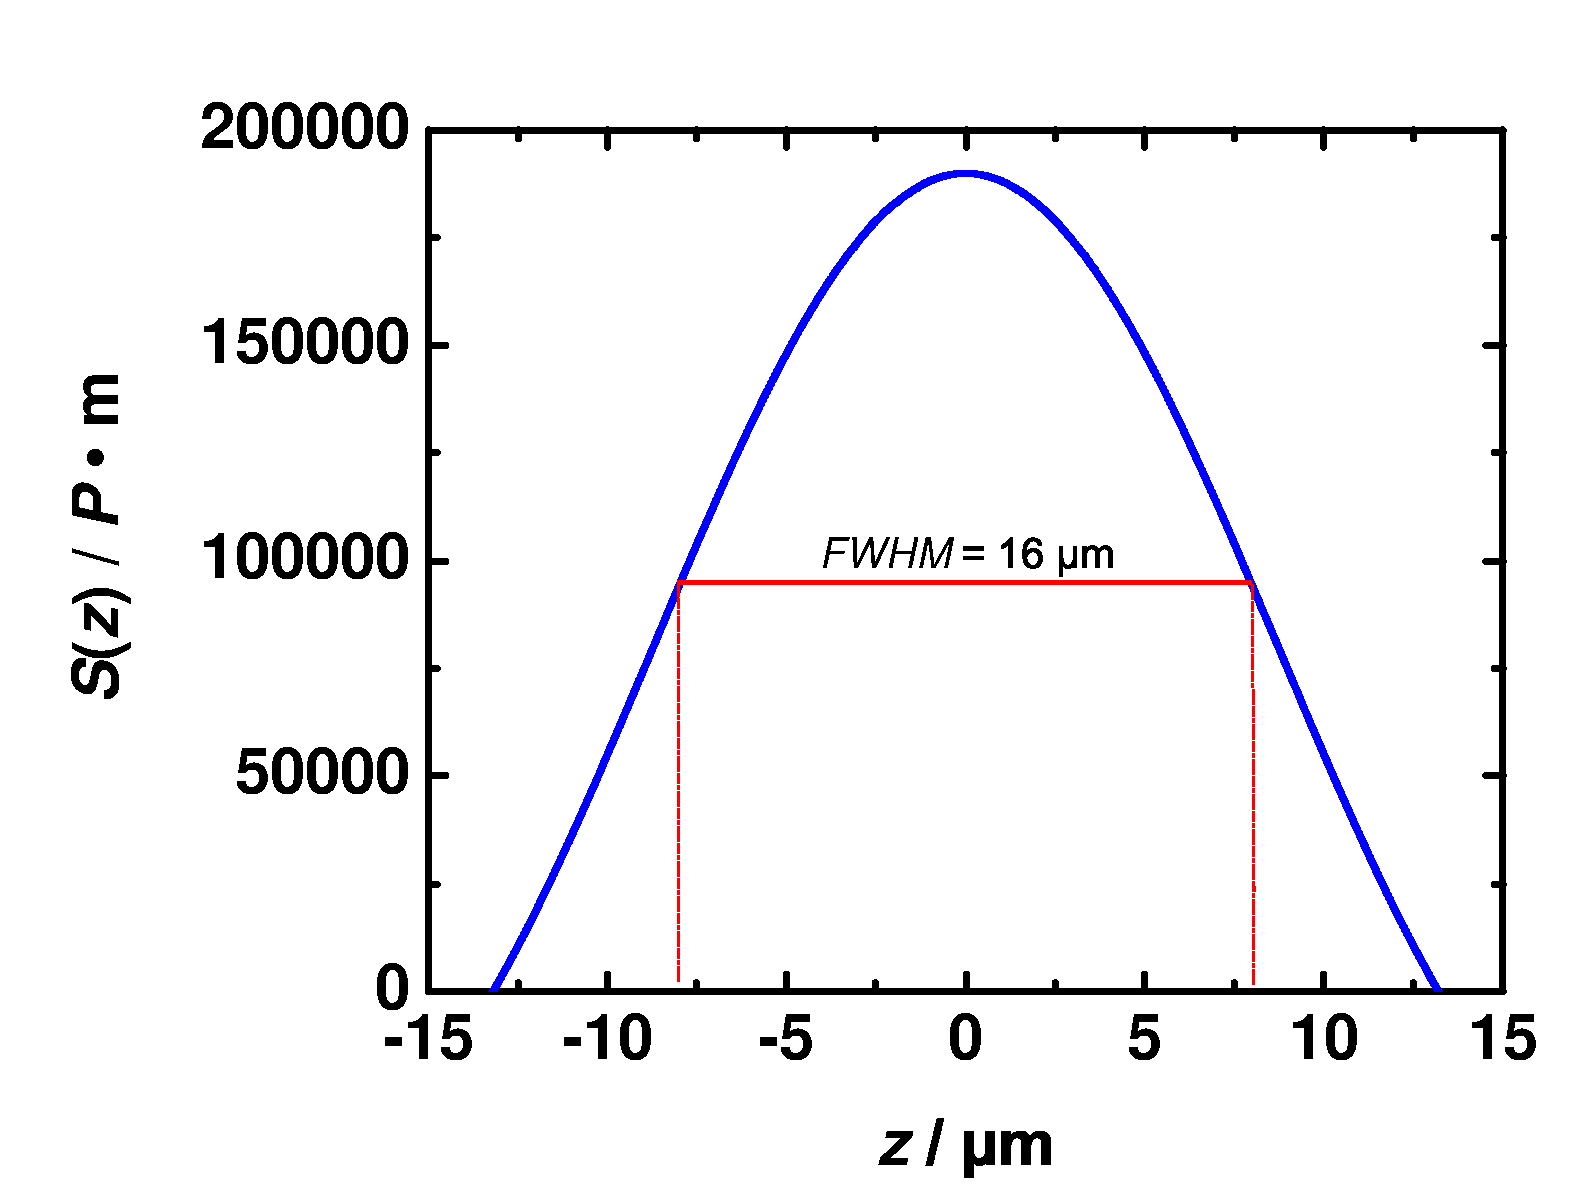
\includegraphics[width=.5\columnwidth]{Grafiken/FWHM.pdf}%
\caption{}%
\label{}%

\end{figure}


\subsection{To which spatial resolution in $\upmu$m in z-coordinates does this correspond?}

\todo{Rayleigh-L�nge?}
\begin{equation}
z_r = \frac{\pi w_0^2}{\lambda}
\label{eq:}
\end{equation}
with the beam waist $w_0$. \todo{$w_0/2$ is FWHM, aber mir ist nicht klar wie ich das gegebene $n$ einbau}

\section{Calculate the depth profile of a spool of adhesive tape}

In a .mat file the measurement of the interface term of a spool of adhesive tape $\breve{u}(k_m)$ is given. To calculate the term in the spacial domain $\breve{u}(z)_{sr}$ the matlab function \verb|fft()| is used. The absolute of the result $\breve{u}(z)_{sr}$ is shown in fig. \ref{fig:profile_nm}.


\begin{figure}[ht]
  \centering
  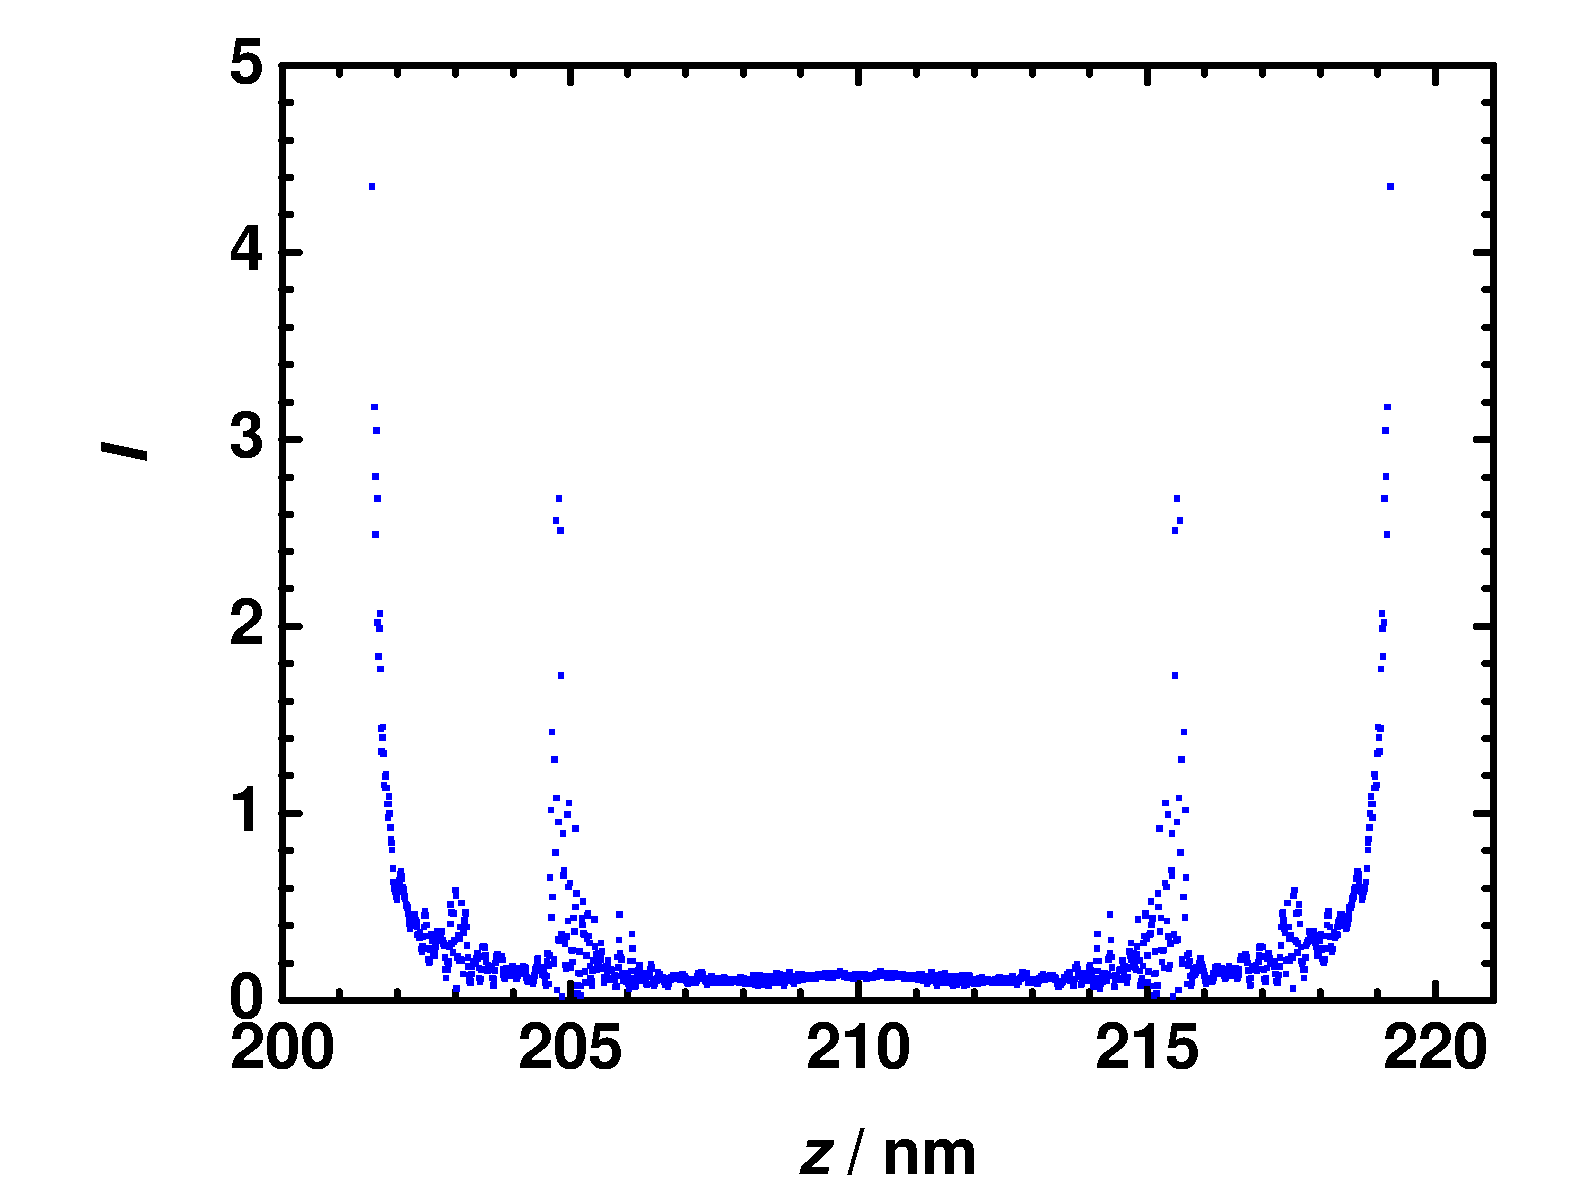
\includegraphics[width=.6\columnwidth]{Grafiken/profile_nm.pdf}

\caption{ }
\label{fig:profile_nm}
\end{figure}


\todo{Stimmt die Gr��enordnung f�r z? Oder muss das Bild noch anders interpretiert werden?}

\begin{equation}
z_m=\frac{2\pi}{k_0-\frac{\Delta k}{2}+m\cdot\delta k}
\label{eq:}
\end{equation}
